
\section{Building Creation}

This is the application of the concepts of Building, Architecture Style and
Facade Attachment defined in section \ref{sec:concepts} Concepts on page \pageref{sec:concepts}.

\subsection{Task Definition}

In order to create a building, the user has to position himself close to the terrain area
where the building is destined to be.
He must then summon a construction plane by invoking the main menu (closed triangle stroke),
choose the create option and do a drop stroke, activating the construction plane gate and
continuing the stroke until the desired position is met.

\begin{figure}[!ht]
		\centering
		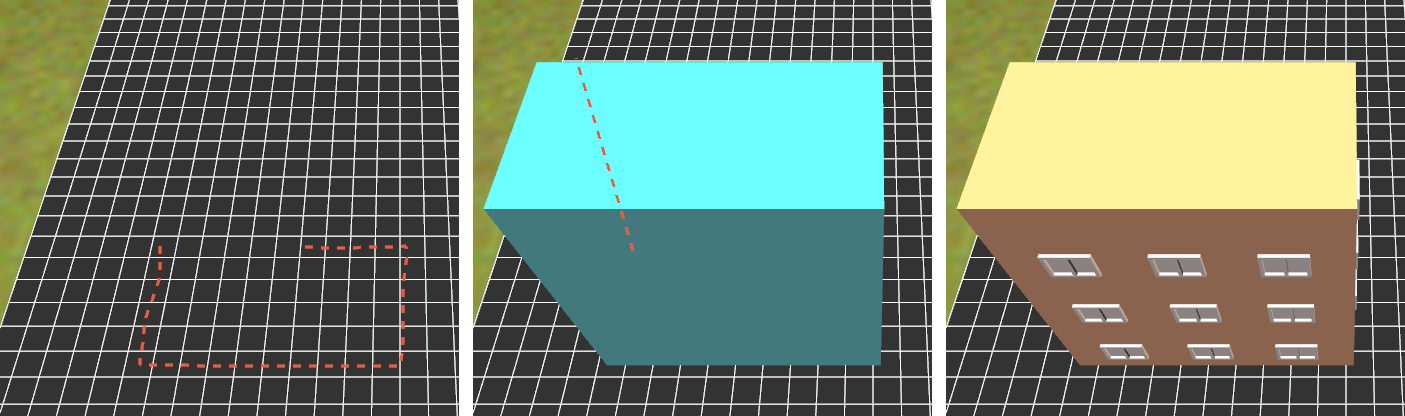
\includegraphics[width=14cm]{gfx/building-creation.png}
		\caption{Building creation steps}
		\label{fig:building-creation}
\end{figure}

%\TODO{ADD STROKE EXAMPLE}

Once the plane is displayed, the user has to draw a stroke resembling a closed rectangle
-- this rectangle defines the blueprint of the facades --
and keep drawing upwards to define the building's height (see figure \ref{fig:building-creation}).

A menu appears then, asking the user for the purpose of this building.
The displayed options are the set of available architecture styles.
The user chooses one and the building's walls are colored and textured,
with facade attachments populating the facade walls and a roof added,
all according to the chosen architecture style.


\subsection{Creation of Facade Attachments}

A facade attachment can be accomplished by modeling an object in Blender,
setting the mesh name to the desired name and applying the export to urban sketcher plug-in 
(see figure \ref{fig:blender-attachment}).
This generates a shape with the format of custom shapes, as described in section \ref{sec:shape-persistence}
on page \pageref{sec:shape-persistence}.
The modeler units are interpreted as meters and the object's origin position should be the facade's floor,
which makes windows have a low origin position, for example.

\begin{figure}[!ht]
		\centering
		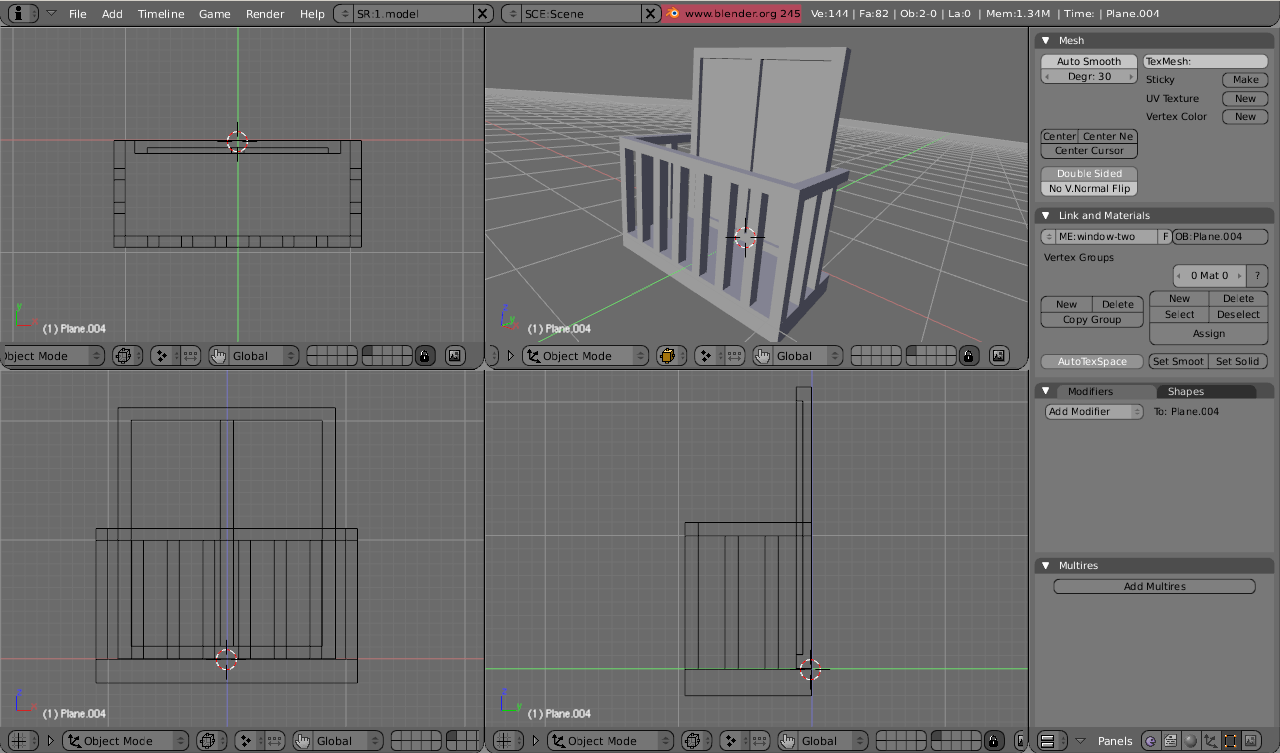
\includegraphics[width=9cm]{gfx/blender-attachment.png}
		\caption{Building creation steps}
		\label{fig:blender-attachment}
\end{figure}

%\TODO{SCREENSHOT?}


%\subsection{Creation of an Architecture Style}

\TODOL{DESCRIBE GRAMMAR}

\TODOL{EXPLAIN POPULATING ALGORITHM}
